% Template for SGN-3507 papers; to be used with:
%          spconf.sty   - ICASSP/ICIP LaTeX style file
%          IEEEtran.bst - IEEE bibliography style file

% Originally created for MCSP 20xx papers;
% Created:  Sep 2006 - Riku Uusikartano -- riku.uusikartano@tut.fi
% Modified: Sep 2007 - Riku Uusikartano -- riku.uusikartano@tut.fi
% Modified: Oct 2009 - Riku Uusikartano -- riku.uusikartano@tut.fi
% Modified: Oct 2010 - Jukka Suhonen -- jukka.suhonen@tut.fi
% Modified: Oct 2011 - Francescantonio Della Rosa -- francescantonio.dellarosa@tut.fi
% Modified: Nov 2011 - Jukka Suhonen -- jukka.suhonen@tut.fi
% Modified for SGN-3507 March 2013 - Juha Pajula -- juha.pajula(a)tut.fi
% Modified for SGN-16006 Jan 2014 - Hanna Silen -- hanna.silen(a)tut.fi

% --------------------------------------------------------------------------
\documentclass{article}

% The amsmath and epsfig packages greatly simplify the process of adding
% equations and figures to the document, and thus their use is highly
% recommended.
% ------------
\usepackage{spconf,amsmath,epsfig}

% Title.
% ------
\title{ SGN-16006, Template for Exercise xyz}



\name{Student, Student
%\thanks{Insert sponsor acknowledgments (where necessary) here.}
}
%
\address{ Student ID number, Student ID number\\
%University / Company\\
%Address\\
email@tut.fi, email@tut.fi}

% Hyphenation (hyphenate all names and non-english words here).
% -------------------------------------------------------------
\hyphenation{Tam-pe-re micro-soft}

\begin{document}

\maketitle
\sloppy

% Abstract.
% ---------
\begin{abstract}
This is a template for the course SGN-16006 -- a slightly modified version of the template of the course SGN-3507. You can use this template or develop your own one. In both cases, the first section of the report, Abstract, should clearly and concisely describe the main results of the task and the aim of the paper. The Abstract appears on the first page, at the top of the left-hand column of text, 11 mm below the title area. It should contain about 100 to 150 words. References should not be introduced in the abstract.
\end{abstract}

% First section, often named as Introduction.
% -------------------------------------------
\section{Introduction}
\label{sec:intro}
This paper provides an example template for the reports of the course SGN-16006 Bachelor's Laboratory Course in Signal Processing. The template is a slightly modified version of the template used at SGN-3507. For the reports of SGN-16006, you can either use this template or develop your own one.

Typically, reports should contain for example the following sections: Introduction, Theory, Methods, Results, and Conclusion. Introduction is used to give an overview and introduction to the topic of the study: what was done and why, what is new in your own approach, etc. Usually a paragraph of metatext describing the contents of the report is given as well. At KIE-34106, a section called Theory (or Background) will be included for the results of the literature review. The following section, Methods, describes how the study was conducted. The outcome of the experiments is described in the section Results. The last section, Conclusion, concludes the paper. Note that sections Theory, Methods, and Results sometimes consist of subsections.

The format of the text of this template is given in the following. The section labels can be different from what was described above; in this case they should be defined according to the contents of the report. Template for \LaTeX and Microsoft Word are available at the course webpage.

The paper size is A4 (210~mm wide by 297~mm tall). All printed material, including text, illustrations, charts, footnotes, and tables, must be kept within a print area of 176~mm wide by 227~mm tall. Do not write or print anything outside the print area.

The top margin must be 35~mm, and the left margin 18~mm.  All text must be in a two-column format. Figures, tables, equations, and such can span two columns, where necessary. The columns are to be 84~mm wide, with a 8-mm space between them.

The font to be used in the text is Times New Roman. The font size for the text is 10 points, and line spacing a single line. The text, including the references, must be justified.

The first paragraph of each section and subsection begins at the left edge of the column. All subsequent paragraphs have a 5-mm indentation in the first sentence.

The sections are numbered, excluding the abstract and the references. The section titles are centered on the columns, and typed in bold 10-point uppercase font. Subsection titles are numbered and left-aligned. The typeface for subsection titles is bold 10 points. Using sub-subsections is discouraged.

The title of the paper is typed using bold 12-point uppercase typeface. The font size for the author name(s) and affiliation(s) is 12 points, the names being in \emph{italic}.

% Optional section.
% ---------------
\section{Theory/Background}
\label{sec:theory}

Theory or the results of the literature review are described here. This section is required in the second report at the course KIE-34106 Academic Writing in English. This section can consist of subsections.


% Second (or third) section.
% ---------------
\section{Methods}
\label{sec:methods}

The methods of the study are described here. These can include, for instance, the methods used for feature extraction and classification. This section can consist of subsections. A description of the format for tables, figures, and equations is given below. Use tables, figures, and equations to clarify the theory or results whenever you find it suitable.

\subsection{Tables}
\label{ssec:tables}

All figures and tables must be numbered. The figure title is centered below the figure, and the table title centered above the table. All the tables and figures should be introduced in the text, for example here: 'Fig.~\ref{fig1} shows a randomly generated hit ratio curve'. A large figure or table can span two columns, when necessary. The correct placement of full page-width figures and tables is on the top of the page.

Tables can be moderately easily constructed using the \LaTeX -commands. An example of a single-column table is shown in Table~\ref{table1}. 


% Example table: some alternative text alignments and cell divisions.
% -------------------------------------------------------------------
\begin{table}[t]
\caption{Example table.}\label{table1}

\begin{minipage}[b]{1.0\linewidth}\centering
\renewcommand{\arraystretch}{1.2}
\begin{center}
\begin{tabular}{l|c|c}
 & Proposed design & Reference design
\\\hline\hline
 Data 1 & 1.12 mm$^2$ & 1.91 mm$^2$\\
\hline
 Data 2 & 32412 & 54213\\
\hline
  \hspace{-6pt}\begin{tabular}{l}Data 3\\[-5pt] (measured) \end{tabular}  & 8.2 mW & 11.3 mW\\
\hline
 Data 4 & \multicolumn{2}{c}{\begin{tabular}{c}some common properties\\[-5pt] for both designs \end{tabular}}\\
\hline
\end{tabular}
\end{center}
\end{minipage}
\end{table}

A large figure or table can span two columns, when necessary. The correct placement of full page-width figures and tables is on the top of the page.


\subsection{Illustrations}
\label{ssec:illustr}
Use figures to clarify and illustrate the theory and results whenever you find it suitable. An example of a single-column figure is shown in Fig.~\ref{fig1}. If possible, figures should be placed on top of the columns. If pdflatex is used for building the pdf-file, used images should be in .pdf or .jpg format.

% Example figure: single-column, width scaled to 84mm (one column width).
% -----------------------------------------------------------------------
\begin{figure}[t]
\begin{center}
  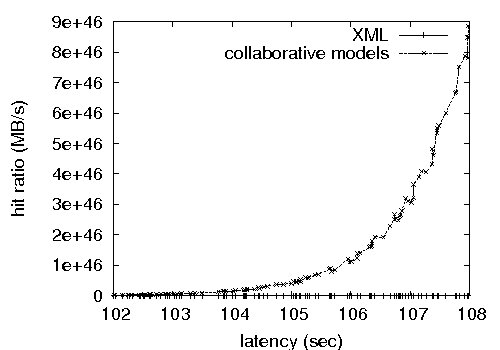
\includegraphics[width=\linewidth]{figure1.jpg}
\end{center}

%\begin{minipage}[b]{1.0\linewidth}\centering
%  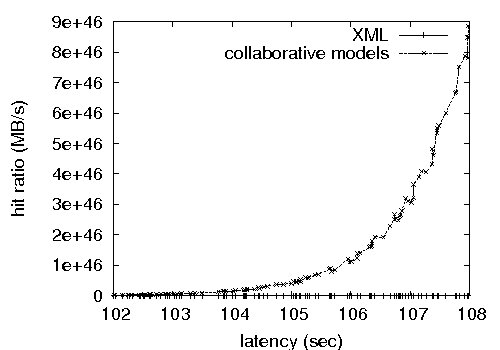
\includegraphics[\width=84mm]{figure1.jpg}
%\end{minipage}
\caption{Randomly generated curve.}\label{fig1}
\end{figure}



\subsection{Equations}
\label{ssec:eq}
Equations are numbered, the equation number being parenthesized and right-aligned. The equation itself is centered on the column and vertically separated from the text by a space of one text line. In the case of multi-line formulas, the equation number is vertically centered on the equation. An example equation \ref{eq:example1} can be written as

%
% Example equation: two lines.
% ----------------------------
\begin{equation}\label{eq:example1}
  H(z) = \frac{z^{-N}(1-z^{-R})^{N}}{(1-z^{-1})^{N}},
\end{equation}
%
where ${N}$ and ${R}$ are some variables, which are typed in $italic$ both in the text and in the equation itself. Note that the equation is a part of a sentence, and thus correct punctuation must be applied. The equations should be written with latex code. Copy-paste images of equations must not be used in the report.

\subsection{Reference Style}
\label{ssec:refstyle}

A high-quality report contains references. Reference style is adopted from IEEE journals and transactions. The style of the TUT thesis writing guide is also accepted. The references are listed in the order they are referenced to in the text. The font size for the references is 9 points.

All references are numbered and formatted using the format adopted by IEEE journals and transactions. The references are listed in the order they are referenced to in the text. The font size for the references is 9 points.

In the \LaTeX environment, the proper format for the references can be easily attained by using the bibtex extension in conjunction with the IEEE reference and abbreviation style files provided on the course web site. Examples of different types of references, such as journals \cite{j:chandrakasan92}, \cite{j:cijvat02}, \cite{j:considine}, \cite{j:polyphase}, \cite{j:vaidyanathan90}, conference papers \cite{c:fettweis99}, \cite{c:yang96}, and patents \cite{p:mecchia02}, are listed in the References section of this paper.

% Third section
\section{Results and discussion}
\label{sec:results}

In the Results section, the found results should be introduced and explained. This section shows how well your algorithm performs, how accurate your classifier is, or how computationally efficient your method is. Do not just list the numerical values or give the result tables/figures; remember to tell the reader how to interpret your results as well!

% Fourth section
\section{Conclusion}
\label{sec:conclusion}

Here, an overview of the study is given: describe what was done and what the main results were.


\small

% IEEEtran is a LaTeX style file defining the reference formatting.
% -----------------------------------------------------------------
\bibliographystyle{IEEEtran}

% IEEEabrv is a LaTeX style file defining the abbreviations of different
% journals and conferences. mcsp_refs contains the actual reference data
% from which the references are selected into the paper using \cite{}.
% ----------------------------------------------------------------------

% Comment of following line if bibliography is not needed
\bibliography{IEEEabrv,mcsp_refs}

% ---------------------------------------------------------------------------
\vfill\pagebreak

\end{document}
